% !TeX spellcheck=en_GB
\RequirePackage[l2tabu, orthodox]{nag}
\documentclass[paper=a4, 12pt]{scrartcl}

\usepackage{graphicx}
\usepackage[font=footnotesize]{caption}
\usepackage[utf8]{inputenc}
\usepackage[colorlinks=true,
	linkcolor=black,
	citecolor=black,
	filecolor=black,
	urlcolor=black]{hyperref}
\usepackage{textcomp}
\usepackage[left=1cm,right=5cm,top=2cm,bottom=2cm,nohead,nofoot]{geometry}
\usepackage[textsize=scriptsize]{todonotes}

\setlength{\marginparwidth}{4cm}

\frenchspacing
\graphicspath{ {../} }

\begin{document}


\noindent
{\huge\sffamily\bfseries NamPRT and NNMT – key drivers of NAD-dependent signalling \par}

\vspace{15mm}

\noindent
Mathias Bockwoldt$^{1}$, Dorothée Houry$^{2}$,  Marc Niere$^{2}$, Toni I. Gossmann$^{3}$, Mathias Ziegler$^{2}$ and Ines Heiland$^{1,\S}$

\vspace{1cm}

\noindent
$^{1}$Department of Arctic and Marine Biology, UiT The Arctic University of Norway, Biologibygget, Framstredet 39, 9017 Tromsø, Norway

\noindent
$^{2}$Department of Molecular Biology, University of Bergen, Thormøhlensgt. 55, 5020 Bergen, Norway

\noindent
$^{3}$Department of Animal and Plant Sciences, Western Bank, University of Sheffield, Sheffield, S10 2TN, United Kingdom

\noindent
§ Corresponding author: ines.heiland@uit.no


\section{Summary}

NAD is best known as cofactor in redox reactions, but it is also substrate of NAD-dependent signalling reactions that consume NAD and release nicotinamide (Nam). In eukaryotes, two different Nam salvage pathways exist. While in lower organisms the initial deamidation of Nam is prevalent, in animals the direct conversion of Nam to the mononucleotide by Nam phosphoribosyltransferase (NamPRT) dominates and eventually remains as the single Nam recycling route in vertebrates.

Strikingly, loss of the deamidation pathway in early vertebrates is preceded by the occurrence of a new enzyme that marks Nam for excretion by methylation – nicotinamide N-methyltransferase (NNMT). The physiological relevance of NNMT is still enigmatic. Why is there an enzyme that removes Nam from recycling, seemingly not having any other physiological role? And why is the occurrence of NNMT accompanied by a diversification of NAD-consuming enzymes?

We have used mathematical modelling approaches to resolve these counterintuitive observations. Our results indicate that NNMT is required to enable high NAD consumption fluxes necessitated by the increasing diversification of NAD-dependent signaling pathways. This kinetic regulation requires a high substrate affinity of the key enzyme for Nam salvage, NamPRT. Indeed, the affinity of NamPRT to Nam has previously been measured to be in the nanomolar range. Mathematical modelling supports the hypothesis that NNMT exerted an evolutionary pressure on NamPRT enforcing the development of its unusually high substrate affinity. Using multiple sequence alignments, we identified a sequence insertion, first occurring in vertebrates, that parallels an – experimentally verified – increase in the substrate affinity of the enzyme. Further simulations show that the deamidation pathway became obsolete owing to the high substrate affinity of NamPRT. Collectively, our results illustrate a close evolutionary relationship between NAD biosynthesis and the diversification NAD-dependent signaling pathways, potentially driven by the concomitant occurrence of a regulator of Nam salvage, NNMT.


\section{Keywords}


%%% TeX-master: "manuscript"
% !TeX spellcheck=en_GB

\section{Introduction}

NAD metabolism has received increasing interest as changes in NAD metabolism are associated with a large number of diseases including but not limited to neurodegeneration, obesity, heart diseases, renal dysfunction and different types of cancer. It has been established that the gradual decrease in NAD during ageing is one of the major driving force of age related pathologies \cite{Chini17}. In addition,  NAD metabolism has emerged as key regulator for axonal degradation \cite{Araki04}. It is therefore not surprising that NAD metabolism and has emerged as promising pharmacological target for disease treatment  \cite{EspindolaNetto2017,Yoshino18, Sinclair18}. However, to develop efficient new therapeutic strategies a better understanding of the pathway dynamics and the pathway components determining it is required.

NAD represents one of the most critical links connecting cellular signal transduction and energy metabolism. Even though it is best known as cofactor for various redox-reactions, NAD is involved in a number of signalling processes that consume NAD$^{+}$ by cleaving the molecule to nicotinamide (Nam) and ADP-ribose \cite{Verdin2015}. These NAD-dependent signalling reactions include poly- and mono-ADP-ribosylation \cite{Butepage2015,DeVos2012}, NAD-dependent protein deacylation by sirtuins \cite{Osborne2016}, and the synthesis of calcium-mobilizing molecules such as cyclic ADP-ribose \cite{Lee2012}. These NAD-dependent signalling processes participate in the regulation of virtually all cellular activities. The enzymes involved in these processes are sensitive to the available NAD concentration \cite{Ruggieri2015}, which in turn is dependent on the NAD$^{+}$/NADH redox ratio. Therefore, NAD-dependent signalling can act as a transmitter of changes in the cellular energy homeostasis, for example, to regulate gene expression or metabolic activity \cite{Koch-Nolte2009}.

The significance of NAD-dependent signalling for NAD homeostasis has long been underestimated. It has now been established, however, that substances affecting NAD biosynthesis lead to a rapid decline of the NAD concentration \cite{Buonvicino2018}. This suggests that NAD-dependent signalling reactions consume substantial amounts of NAD. Therefore, we hereafter refer to them also as NAD-consuming reactions. The resulting NAD turnover differs in a cell-type-specific manner and can lead to an NAD half-life as short as 15 minutes \cite{Liu2018}. To maintain the NAD concentration at physiological levels, NAD biosynthesis needs to act at an equally rapid rate. Imbalances in NAD homeostasis have been linked to various mainly age related diseases, such as diabetes, neurodegenerative disorders, and cancer \cite{Chiarugi2012,Verdin2015}. Several recent studies have demonstrated impressive health benefits of dietary supplementation with intermediates of NAD biosynthesis including Nam mononucleotide (NMN) and Nam riboside (NR) \cite{Yoshino2018}. Apparently, the exploitation of NAD biosynthetic routes, in addition to the use of nicotinamide as precursor (fig.~\ref{fig:pathway_overview}), results in increased NAD concentrations that stimulate NAD-dependent signalling processes, in particular, protein deacetylation by sirtuins \cite{North2004}.

Due to the constant release of Nam through NAD-consuming signalling reactions, the NAD salvage pathway using Nam as precursor is the most important NAD synthesis pathway. In general, two principal pathways exist that recycle Nam.  Vertebrates use a direct two-step pathway starting with the conversion of Nam into the mononucleotide NMN by the Nam phosphoribosyltransferase (NamPT) using phosphoribosyl pyrophosphate (PRPP) as co-substrate. The nearly complete recycling of Nam by NamPRT is achieved by an extraordinary high substrate affinity to Nam, the $K_{M}$ being in the low nanomolar range \cite{Burgos2008}. This appears to be mediated by an ATP-dependent phosphorylation of a histidine residue in the catalytic core \cite{Burgos2009}. Despite the importance of its salvage, Nam can also be marked for excretion by methylation. The presence of nicotinamide N-methyltransferase (NNMT) in vertebrates \cite{Gossmann2012FEBS} is among the most enigmatic and counterintuitive features of NAD metabolism. While NamPRT is seemingly optimised to recycle even the faintest amounts of Nam back into NAD synthesis, NNMT seems to have no function other than to remove Nam from NAD metabolism. It has been suggested that the process potentially acts as a metabolic methylation sink \cite{Pissios2017}.

In most prokaryotes as well as in plants and fungi, another pathway consisting of four steps starting with the deamidation of Nam to nicotinic acid (NA) by the Nam deamidase (NADA) is used. (fig.~\ref{fig:pathway_overview}). The three enzymes that act after NADA belong to the Preiss-Handler pathway that also exists in vertebrates. NA is converted into the corresponding mononucleotide (NAMN), in a reactions performed by the NA-specific phosphoribosyltransferase NAPRT. The conversion of both mononucleotides, NMN and NAMN, into their corresponding dinucleotides, NAD and NAAD, is catalysed by the Nam/NA adenylyltransferases (NMNATs) that are essential in all organisms \cite{DeFigueiredo2011}. The recycling pathway via NA finally requires re-amidation of NAAD by NAD synthase. This final reaction includes an enzyme adenylation step that consumes ATP. Therefore, the Nam recycling by NADA appears to be energetically less efficient than the recycling pathway starting with NamPT.

We and others have earlier shown that the two NAD biosynthesis pathways starting from Nam co-exists in some eukaryotes \cite{Gossmann2012FEBS,Carneiro2013}, as well as in some bacterial species \cite{Gazzaniga2009}. Why these pathways co-exists in some organisms and over a very long evolutionary time frame and why NADA nevertheless disappears in vertebrates, is not known. We furthermore have little understanding of the physiological role of NNMT and its impact on NAD-metabolism so far.

As earlier analyses have been limited by the few eukaryotic genomes available at the time, we here performed a comprehensive phylogenetic analysis of the NAD pathways using 793 eukaryotic and 7892 prokaryotic genomes. Our results suggest that there has been a selection for the co-existence of NamPRT and NNMT in deuterostomes, while the deamidation pathway, which is dominant in bacteria, became superfluous. This transition was accompanied by a marked increase in the number of NAD-consuming signalling enzymes. Mathematical modelling of the pathway revealed an unexpected positive kinetic role of NNMT for NAD-consuming signalling fluxes, through prevention of accumulation of Nam. In addition, the model predicts that NNMT likely exerted an evolutionary pressure on NamPT to develop a high affinity towards its substrate Nam. Indeed, we identified a short sequence insertion in NamPT, which first occurs in Deuterostomes and that appears to modulate the affinity of NamPT. Simulating the resource competition, we furthermore show that the presence of high affinity NamPT together with NNMT makes the NADA-dependent pathway obsolete.

Taken together, our analyses suggest that the co-existence of NamPT and NNMT has been a prerequisite to enable the evolutionary development of versatile NAD-dependent signalling mechanisms present in vertebrates.


%%% TeX-master: "manuscript"
% !TeX spellcheck=en_GB

\section{Results}

\subsection{Paradoxical evolutionary correlation between NAD-dependent signalling and precursor metabolism}

\todo[inline]{MZ: Ich finde, die NAD-abhängigen Signalwege kommen in den Resultaten zu kurz weg. Es genügt vielleicht, einfach die 10 Klassen noch mal aufzuzählen (also z.B. x verschiedene PARP-Klassen, y Sirtuin-Klassen usw.). Dies würde ich gegenüberstellen an den Stellen, wo große Sprünge passieren. Daraus kann man z.B. ablesen, an welchen Stellen sich welche Signalwege speziell weiterentwickelt/diversifiziert haben. MB: Ich versuch mal, die entsprechenden Infos aus den Ergebnissen zu bekommen.}

To understand the functional roles and potential interplay between the three known enzymes that use Nam as substrate (NamPRT, NADA and NNMT), we first conducted a comprehensive phylogenetic analysis. The phylogenetic distribution of the two enzymes that initiate the two different NAD salvage pathways, NADA and NamPRT is scattered in bacteria \cite{Gazzaniga2009}, while their co-occurrence has been detected in some marine invertebrates \cite{Gossmann2012FEBS}. As shown in Figure~\ref{fig:phylo_distribution}A, bacteria, fungi, and plants predominantly possess NADA and only a few of them harbour NamPRT. In contrast, Metazoa predominantly lost NADA and have NamPRT together with NNMT. NNMT seems to have arisen \textit{de~novo} in the most recent common ancestor of Ecdysozoa and Lophotrochozoa (fig.~\ref{fig:phylo_distribution}B). We were unable to find any \textit{NNMT} gene with an e-value below 0.1 in fungi or plants.

Nematodes are the only organisms, where we observed a concomitant presence of NADA and NNMT. In deuterostomes, the only large clade that possesses only NamPRT and seems to have lost NNMT are Sauropsida, and among them especially birds. The reason why about half of the sequenced bird genomes do not seem to encode for NNMT remains unclear. The distribution of NNMT in birds is quite scattered (suppl. fig.~S2). \todo{figure not corresponding to current species tree \cite{Prum2015}. MB: Will recreate this figure with the tree from the paper asap.} The lack of NNMT might be related to the excretion system, as the product of NNMT, methyl-Nam, is in mammals excreted with the urine. There are few metazoan species for which we could not find NamPRT or NADA, while NNMT was present. We assume that this is due to incomplete genomes in the database, as the distribution of such species is scarce and widely scattered.

In addition to the phylogenetic distribution of the two Nam salvage enzymes NADA and NamPRT, we analysed the phylogenetic diversity of enzymes catalysing NAD-dependent signalling reactions. To do so, we used the previously established classification into ten different families of NAD-consuming signalling enzymes \cite{Gossmann2012FEBS}. The detailed list of templates used for the phylogenetic analyses can be found in supplementary table~S1. The numbers shown in figure~\ref{fig:phylo_distribution}B denote the average number of NAD-dependent signalling enzyme families found in each clade. With the exception of Cnidaria and Lophotrochozoa, we find an average of three to four families in protostomes, whereas most deuterostome species have, on average, more than eight families with an increasing diversification of enzymes within some of these families \cite{Gossmann2014DNAR}.

Taken together, we found that NADA is lost in vertebrates, but strongly preserved in most other organisms, despite the higher energetic requirement of that pathway. Moreover, the selection for having both NamPRT and NNMT coincides with an increased diversification of NAD-dependent signalling. This observation seems counterintuitive, as one would expect that increased NAD-dependent signalling should be accompanied by an increase of substrate availability for NAD biosynthesis.


\subsection{Functional properties of NamPRT and NNMT have evolved to maximize NAD-dependent signalling}

To resolve this apparent contradiction, we wished to scrutinize the NAD metabolic network. Given the complexity of this network, we turned to modelling approaches and built a dynamic model of NAD metabolism based on previously reported kinetic data (for details, see experimental procedures and suppl. tab.~S2).

To be able to compare metabolic features of evolutionary quite different systems in our simulations and as we had limited information about expression levels of enzymes, we initially used equal amounts for all enzymes. As we have very few cross species kinetic data, we were furthermore mainly relying on kinetic constants found for human or yeast enzymes. Wherever possible, we included both substrate affinities and known product inhibitions or inhibition by downstream metabolites. As we in addition assumed that cell growth is, besides NAD-consuming reactions, a major driving force for NAD biosynthesis, we analysed different growth rates (cell division rates) by simulating different dilution rates for all metabolites.

First, we addressed the unexpected correlation between the selection for co-occurrence of NamPRT and NNMT and an increase in the number of NAD-consuming enzyme families. We calculated steady state NAD concentrations and NAD consumption rates by simulating NAD biosynthesis proceeding via NamPRT in the presence or absence of NNMT. To achieve free NAD concentrations in the range reported in the literature and due to the very low turnover of NamPRT, we used tenfold higher NamPRT levels compared to other enzymes. We also adjusted the amount of NMNAT accordingly to avoid that the NAD synthesis rates are limited by this enzyme. Surprisingly, as shown in figure~\ref{fig:NNMT_NAD_flux}, the presence of NNMT enables higher rather than lower NAD consumption rates (fig.~\ref{fig:NNMT_NAD_flux}A). However, it diminishes the steady state concentration of NAD (fig.~\ref{fig:NNMT_NAD_flux}B). The decline in NAD concentration can be compensated by a higher expression of NamPRT, further increasing NAD consumption flux (dashed lines in fig.~\ref{fig:NNMT_NAD_flux}A and~B).

These results can be explained by looking in more detail at the kinetic parameters of NamPRT and NAD-consuming enzymes such as Sirtuin~1. Most NAD-consuming enzymes are inhibited by their product Nam. Thus the presence of NNMT enables higher NAD consumption fluxes, by removing excess Nam from the cells. At the same time, the high substrate affinity of NamPRT maintains a sufficiently high NAD concentration, although the concentration is, as expected, lower than in the system without NNMT.

Kinetic paramters of NamPRT were previously meassured for the human enzyme \cite{Burgos2008} as well as for some bacterial enzymes\todo{insert ref}, the latter having a much lower substrate affinity for Nam. We thus analysed the potential effect of NamPRT affinity ($K_{M}$) on NAD steady state concentration and NAD consumption flux. In the absence of NNMT, a variation of the substrate affinity of NamPRT for Nam, has very little effect on steady state NAD concentration and NAD consumption flux (fig.~\ref{fig:NamPRT_affinity_Nam}A and~B). In the presence of NNMT, however, NAD consumption flux and NAD concentration increases with decreasing $K_{M}$ values of NamPRT (fig.~\ref{fig:NamPRT_affinity_Nam}C and~D).

Remarkably, NAD concentration and consumption flux are both considerably affected by cell division rates in a system without NNMT, at least if the enzyme expression is kept constant at different cell division rates. Of course, this is an artificial scenario, as one would assume organisms to regulate enzyme expression to achieve similar levels of metabolite concentrations instead. Nevertheless, in the absence of NNMT there seems to be a trade-off between maintainable NAD concentration and consumption flux. In contrast, in the presence of NNMT, NAD consumption rates and concentrations are almost independent of cell division rates.

Figures~\ref{fig:NamPRT_affinity_Nam}E and~F visualise a direct comparison of simulations assuming different affinities of NamPRT for Nam, in the presence or absence of NNMT. Interestingly, at an affinity of $K_{M}$ =~1\,$\mu$M, which is in the range of the $K_{M}$ of NADA for Nam, NAD consumption flux is only higher with NNMT present when cell division rates are low (fig.~\ref{fig:NamPRT_affinity_Nam}E). If the affinity of NamPRT is high enough, consumption rates are always higher with NNMT than without it. The NAD concentration is always lower with NNMT (fig.~\ref{fig:NamPRT_affinity_Nam}F).

To understand the interplay and competition for Nam between NNMT and NamPRT, we scanned a wide range of possible $K_{M}$ values for both enzymes in our simulations. As shown in figure~\ref{fig:optimal_substr_affinities}, the simulations indicate that both NAD consumption flux and NAD concentration would be minimal in case of a high $K_{M}$ for NamPRT and a low $K_{M}$ for NNMT. Conversely, lowering the $K_{M}$ of NamPRT to the nanomolar range substantially increases NAD consumption and concentration, which reach a maximum when the $K_{M}$ of NNMT is concomitantly elevated to the submillimolar range. The asterisks in figure~\ref{fig:optimal_substr_affinities} denote the $K_{M}$ values actually found for the human enzymes. Astonishingly, the naturally occurring $K_{M}$ values are very close to the theoretical optimum.


\subsection{Sequence variance acquired in metazoans enhances substrate affinity}

Given that NNMT might have exerted an evolutionary pressure on the development of NamPRT, one would expect to observe adaptations that are reflected in the NamPRT protein sequence arising with the occurrence of NNMT. To explore this, we created a multiple sequence alignment. The alignment of selected sequences is shown in figure~\ref{fig:unresolved_loop}A and a more comprehensive multiple sequence alignment containing a larger number of species can be found in supplementary figure~S1. We found that most Deuterostomes that possess only NamPRT and NNMT (indicated by the blue circle) have an insert of ten amino acids corresponding to positions 42 to 51 in the human enzyme. This insert overlaps with a predicted weak nuclear localisation signal (NLS), that is lost when the insert is removed. These ten amino acids correspond to a stretch at the protein surface that is unresolved in all available crystal structures of human NamPRT (e.g. structure visualisation in fig.~\ref{fig:unresolved_loop}B from \cite{Wang2006}). Intriguingly, this presumed loop, depicted in red in figure~\ref{fig:unresolved_loop}B, is connected to one of the $\beta$-sheets involved in substrate binding \cite{Burgos2009} and in the functional homodimer, the two loops are placed side-by-side.

From these observations, we derived two possible hypotheses regarding the role of the loop in NamPRT function. The first hypothesis was that the presence of the loop could change the subcellular localisation of NamPRT, as it is overlapping with a predicted NLS. To test this hypothesis, we created a mutant NamPRT lacking the loop and recombinantly expressed FLAG-tagged wildtype and mutant NamPRT in HeLa S3 cells. Immunofluorescence imaging showed a mixed cytosolic nuclear localisation for both the wildtype and the mutant NamPRT (fig.~\ref{fig:unresolved_loop}C). Thus, deletion of the loop did not compromise the nuclear localisation.

The second hypothesis was that the sequence insertion might influence substrate binding of NamPRT. We thus expressed both wildtype and mutant proteins, N-terminally fused to a 6xHis-tag in \textit{E.~coli}, and purified them. The size exclusion chromatography profile showed that both wildtype and mutant protein were expressed as dimers (see suppl. fig.~S3), indicating that the missing residues in the mutant did not dramatically affect the protein structure. The enzymatic activity was measured by NMR spectroscopy using the detection of NMN produced in the presence and absence of ATP. Upon incubation with the NamPRT inhibitor FK866 \cite{Hasmann2003} for 30 minutes, both wildtype and mutant NamPRT did not produce any NMN, suggesting that binding of FK866 is not affected by the mutation (see suppl. fig.~S4). Nevertheless, the enzymatic activity of the mutant enzyme was only approximately ... percent \todo{insert number} of that of the wildtype enzyme (fig.~\ref{fig:unresolved_loop}D). In contrast to wildtype NamPRT, the activity of the mutant enzyme was not stimulated in the presence of ATP (fig.~\ref{fig:unresolved_loop}E). These observations suggest that the mutant enzyme is catalytically active, retains its dimeric state and sensitivity to FK866. However, the lower activity and the absence of catalytic activation by ATP indicate that deletion of amino acids 42 to 51 might have affected substrate binding.


\subsection{NamPRT and NNMT made NADA obsolete in vertebrates}

Next, we wished to understand why NADA was lost in vertebrates. As selection during evolution results usually from competition for resources, we built a two compartment model, based on the pathway model described above. One compartment contains NADA, while the other one contains either NamPRT alone or together with NNMT. Both compartments share a limited Nam source (for details, see experimental procedures and suppl. tab.~S2). Without NNMT, the compartment containing NADA shows slightly lower NAD consumption rates (fig.~\ref{fig:NNMT_comp_advantage}A), but is able to maintain much higher NAD concentrations especially at low cell division rates (fig.~\ref{fig:NNMT_comp_advantage}B). At high cell division rates, steady state concentrations in both compartments are similar. This might explain why in bacteria, that often have relatively high growth rates, both systems can co-exist.

In the presence of NNMT, the NamPRT compartment has both higher NAD consumption rates and higher steady state NAD concentrations than the compartment containing NADA (fig.~\ref{fig:NNMT_comp_advantage}C and~D). The higher NAD concentrations in the compartment containing NamPRT and NNMT can, however, only be maintained if the affinity of NamPRT for Nam is high enough. If the substrate affinity of NamPRT is too low (high $K_{M}$), the NADA compartment is able to maintain higher NAD concentrations, but still has a lower NAD consumption flux. Taken together, the results suggest that the NADA pathway might have become obsolete upon emergence of the high affinity NamPRT. This in turn might have been induced by the appearance of NNMT.


%%% TeX-master: "manuscript"
% !TeX spellcheck=en_GB

\section{Discussion}

We here comprehensively analysed the phylogenetic distribution of the three enzymes using Nam as a substrate. These are the two NAD salvage pathway enzymes NADA and NamPRT as well as the Nam-degrading enzyme NNMT. We found that after the first appearance of NNMT in Protostomia, a diversification of NAD-consuming reactions in Deuterostomia can be observed. We could explain these finding using mathematical modelling, as NNMT removes excess Nam from cells and thereby reduces product inhibition of NAD signalling enzymes. This in turn enables higher fluxes through these reactions. Thus, the diversification of NAD-consuming enzymes in mammals seems to have been enabled by the presence of NNMT.

NAD-consuming enzymes are involved in a wide variety of signalling and gene regulatory mechanisms that, due to their sensitivity to NAD$^{+}$, have the ability to translate differences in metabolic states into changes in signalling and gene regulation. As NAD concentrations are lowered by the removal of NAD precursor by NNMT,  a high affinity of NamPRT is required for high NAD consumption fluxes and NAD concentrations in the presence of NNMT. It therefore seems plausible that NNMT might have been driving NamPRT evolution. Looking at the enzyme affinities of the human enzymes, it furthermore appears that both NNMT and NamPRT reached an almost optimal state, as further changes in the affinity of either NamPRT or NNMT would not result in much higher steady state NAD concentrations or NAD consumption fluxes. In addition, our simulations suggest that NNMT makes both NAD concentration and NAD consumption relatively independent of other processes requiring NAD, such as cell growth.

Our findings shed new light on the potential physiological role of NNMT, which has earlier been recognised as potential marker for some types of cancer \citep[e.g.][]{Okamura1998}. The main healthy tissue expressing NNMT is the liver, while no or only little expression of NNMT is observed in most other healthy tissues \citep{Aksoy1994}. The increased NNMT expression observed in some types of cancer, might serve to remove Nam derived by increased NAD-dependent signalling. To maintain high NAD concentrations, a simultaneous higher expression of NamPRT is required, which is what has been found in some types of cancer \citep{Bi2011,Wang2011}. It is worth noticing, that NNMT is only advantageous as long as NamPRT affinity is sufficiently high. This suggests that certain types of cancer expressing NNMT at a high level, would potentially be more susceptible to competitive inhibitors of NamPRT. Several of such inhibitors are currently tested in clinical studies \citep{EspindolaNetto2017,Xu2015SR}. Based on our analysis, we would suggest that it might be reasonable to screen patients before treatment, as non-NNMT expressing tumours might respond less to competitive NamPRT inhibitors and missing Nam degradation in those cancer cells would potentially lead to an accumulation of Nam that could outcompete the inhibitor. The latter aspect is not well investigated and requires further analysis.

Neither the scattered distribution of NamPRT and NADA that is especially pronounced in bacteria \citep{Gazzaniga2009}, but that has also been observed in eukaryotes, nor the disappearance of NADA in vertebrates has been understood earlier. Our combined phylogenetic-modelling analysis now provides a potential explanation for both observations. Using simulated competition between two compartments that share the same limited source of Nam, we show that the compartment that contains NamPRT and NNMT can maintain a higher steady state NAD concentration and NAD consumption rate than the compartment containing NADA. This is, however, only the case if NamPRT substrate affinity is sufficiently high. The dominant enzyme combination found in vertebrates, a high-affinity NamPRT with NNMT, thus seems to provide a competitive advantage. As this may also hold for mammalian-associated bacteria, particularly pathogens, we wanted to see whether pathogenic bacteria solely express NamPRT. Unfortunately, bacterial habitat information is currently far from complete and often difficult to access. We therefore manually checked bacteria that possess NamPRT and indeed found that most of them have been characterised to be pathogenic. It should be noted that the distribution of NADA and NamPRT does not follow the bacterial species tree \citep{Gazzaniga2009}. Besides the suggestion made here, there might well be other environmental aspects that influence the phylogenetic distribution in bacteria.

A detailed analysis of sequence variances in NamPRT revealed that only deuterostomes that have NNMT, but not NADA, have a sequence insertion in the N-terminal part of NamPRT that seems to enable the high affinity of the enzyme. This in turn would suggest that also the bacterial enzymes do not have a high substrate affinity. The substrate affinity measured for a bacterial NamPRT from \textit{Acinetobacter baylyi} \citep{Sorci2010} is indeed 10\,000 times higher lower ($K_{M}$ of 0.04mM) than that of the human NamPRT, supporting our hypothesis. Other bacterial NamPRTs were shown to be functional \citep{Martin2001,Gerdes2006}, but the substrate affinities have not been determined. The differences in activity and affinity, implying differences in substrate binding could potentially be exploited for the development of antibiotics. Further analysis possibly including the crystallisation of a bacterial NamPRT would be required, to see whether the bacterial NAD metabolism could be a promising target.

% Martin2001: Haemophilus ducreyi: no kinetic measurements
% Sorci2010: Acinetobacter sp.: NamPRT (Nam) Km: 0.04 mM (= 40 000 nM); kcat: 0.12/s (apparent values determined at constant 5 mM PRPP and 2 mM ATP)
% Gerdes2006: Synechocystis sp.: only activity 0.5 U/mg NamPRT for Nam
% Human, according to table S2: Km: 5 nM; kcat: 0.0077/s

In our analyses, we did not consider the potential effects of co-substrates of the investigated pathway. Such co-substrates include targets of the NAD-consuming enzymes, such as acylated proteins for sirtuins, for example, or phosphoribosyl pyrophosphate (PRPP) and ATP that are required for NMN synthesis by NamPRT. Furthermore, the presence of the methyl donor \textit{S}-adenosyl methionine (SAM) and its precursor methionine that have been shown to potentially limit the effect of NNMT \citep{Ulanovskaya2013} was not considered here. As co-substrate availability might alter the behaviour of the system, these should thus be included in future analyses. Unfortunately, information about the \textit{in~vivo} concentrations of these co-substrates is currently very limited.

During our analysis, we came across several problems related to the use of NCBI sequence databases for phylogenetic analyses. One is sequence contamination, which is a well-known problem \citep{Ballenghien2017,Longo2011}. To avoid contamination, we used sequence homology analysis to remove all sequences of obvious bacterial origin from the results in eukaryotic species. Another problem is incomplete genomes. Although there are tools to assess the completeness of a genome \citep[e.g.][]{Simao2015}, none of them could convincingly claim to be reliable. The genomes of the common model organisms can probably be assumed to be close to complete, but there are many draft genomes in the databases whose completeness is uncertain. Even if the completeness would be known, due to the high number of genomes used in this analysis, it is likely that some genes of interest were not sequenced in every genome. For our analysis, this means that scattered patterns of few missing genes could be real, but are in general thought more likely to stem from an incomplete genome.

The third problem are wrong annotations. We tried to avoid these, by only relying, wherever possible,  on template sequences with confirmed function. This problem becomes apparent by the fact that in yeast an enzyme named NNMT can be found. The initial naming was based on a very weak homology to human NNMT and an analysis of life span extension of the mutant in \textit{Saccharomyces cerevisae} \citep{Anderson2003}, which showed similar effects as other mutants of the NAD pathway. The protein has later been shown not to function as methyltransferase for Nam, but for the eukaryotic elongation factor~1A (eEF1A) giving it its new name elongation factor methyltransferase~7 (Efm7) \citep{Hamey2016}. The old name is still present in many databases, though.

Taken together, we have been able to comprehensively analyse the functional co-evolution of several enzymes of the NAD pathway. The appearance of NNMT seemingly initiated and drove complex alterations of the pathway such as an increase and diversification of NAD-dependent signalling, followed by an increase in NamPRT substrate affinity. A schematic overview is given in figure~\ref{fig:evo_events}. This transition appears to be accompanied by the loss of NADA in vertebrates and the first gene duplication of NMNATs \citep{Lau2010}. We also noted that the second gene duplication of NMNATs and thus the further compartmentalisation of NAD metabolism is co-occurring with a site-specific positive selection event in NNMT (unpublished results).

We here developed a new approach that combines detailed phylogenetic analysis with dynamic metabolic modelling and have been able to explain observed evolutionary changes in the NAD biosynthesis and consumption pathway. Based on the simulated pathway dynamics, we have furthermore derived predictions for physiological interdependencies between several enzymes of the pathway that are potentially relevant for new disease treatments. Our results, including the experimental verification of parts of our predictions, demonstrate the potential of our approach for the analysis of dynamic networks and how the approach can be used to unravel functional interdependencies within pathways of interest.


%%% TeX-master: "manuscript"

\section{Experimental Procedure}

\subsection{Dynamic modelling}

Kinetic parameters (substrate affinity (Km) and turnover rates (kcat), substrate and product inhibitions) were retrieved from the enzyme database BRENDA and additionally evaluated by checking the original literature especially with respect to measurement conditions. Parameter values from mammals were used if available. For enzymes not present in mammals, values from yeast were used. The full list of kinetic parameters including reference to original literature can be found in Supplementary table 1. For NMNAT, the previously developed rate law for substrate competition was used \cite{Schauble2013}. Despite these modifications, Henri-Michaelis-Menten kinetics were used for all reactions except the import and efflux of Nam, which were simulated using constant flux and mass action kinetics, respectively. All simulations were performed using the steady state calculation and parameter scan options provided by COPASI 4.22 \cite{Hoops2006}. The model will be available at the Biomodels database accession number xxx\todo[author=Ines]{Insert number}. Related figures were generated using gnuplot\todo[author=Ines]{Version?}.


\subsection{Phylogenetic Analysis}

NADA, NamPRT, and NNMT enzymes or enzyme candidates were identified using Blastp with known enzymes against the NCBI non-redundant protein sequence database (nr). A list of functionally verified enzymes used as templates is given in supplementary table 2. This table also includes the length cut-offs for identified enzymes. The e-value cut-off was 1e-30 for all enzymes. Blastp parameters were set to yield maximum 20\,000 target sequences, using the BLOSUM62 matrix with a word size of 6 and gap opening and extension costs of 11 and 1, respectively. Low-complexity filtering was disabled. Obvious sequence contaminations were removed by manual inspection of the results. The taxonomy IDs of the species for each enzyme was derived from the accession2taxonomy database provided by NCBI. Scripts for creating, analysing, and visualising the phylogenetic tree were written in Python, using the ETE3 toolkit (Huerta-Cepas, 2010).


\subsection{Generation of eukaryotic expression vectors encoding C-terminally FLAG-tagged NamPRT proteins}

The open reading frame (ORF) encoding human NamPRT was inserted into pFLAG-CMV-5a (Merck - Sigma Aldrich) via EcoRI/BamHI sites. Using a PCR-based approach, this vector provided the basis for the generation of a plasmid encoding a NamPRT deletion mutant lacking amino acid residues 42-51 (NamPRT-$\Delta$42-51). The sequences of the inserted ORFs were verified by DNA sequence analysis.


\subsection{Transient transfection, immunocytochemstry, and confocal laser scanning microscopy}

HeLa S3 cells cultivated in Ham’s F12 medium supplemented with 10\% (v/v) FCS, 2\,mM L-glutamine, and penicillin/streptomycin, were seeded on cover slips in a 24 well plate. After one day, cells were transfected using Effectene transfection reagent (Qiagen) according to the manufacturer’s recommendations. Cells were fixed with 4\% paraformaldehyde in PBS 24 hours post transfection, permeabilised (0.5\% (v/v) Triton X-100 in PBS) and blocked for one hour with complete culture medium. After overnight incubation with primary FLAG-antibody (mouse M2, Sigma-Aldrich) diluted 1:2500 in complete medium, cells were washed and incubated for one hour with secondary AlexaFluor 594-conjugated goat anti mouse antibody (ThermoFisher, Invitrogen) diluted 1:1000 in complete culture medium. Nuclei were stained with DAPI and the cells washed. The cover slips were mounted on microscope slides using ProLong Gold (ThermoFisher, Invitrogen). Confocal laser scan imaging of cells was performed using a Leica TCS SP8 STED 3x microscope equipped with a 100x oil immersion objective (numerical aperture 1.4).


\subsection{Generation of bacterial expression vectors encoding mutated or wildtype NamPRT proteins}

BL21-codonPlus (DE3) RIL cells were transformed with pQE-30 NamPRT WT/pREP4 or pQE-30 NamPRT $\Delta$42-51/pREP4. Bacterial cells were grown at 37\,°C in 250\,rpm shaking incubator in 1\,L of LB medium containing 100\,µg/mL ampicillin, 50\,µg/mL kanamycin, and 32\,µg/mL chloramphenicol. Protein expression was induced with 0.2\,mM isopropyl-$\beta$-D-thiogalactoside (IPTG) at an OD600 of 0.4 to 0.6. Induction was done overnight at 18\,\textdegree C in 250\,rpm shaking incubator.


\subsection{Purification of NamPRT}

The cells were harvested by centrifugation and resuspended in lysis buffer (20\,mM Tris-HCl pH 8.0, 500\,mM NaCl, 4\,mM dithiltheritol (DTT), 1\,mg/mL lysozyme, 1X Complete EDTA-free protease inhibitor cocktail (Roche)). After sonification, the lysate was centrifuged for 30\,min at 13000\,g, and the clear lysate was incubated with 2\,mL of Nickel-NTA resin (Qiagen). Non-specific protein binding was removed with washing buffer (20\,mM Tris-HCl pH 8.0, 500\,mM NaCl, 1\,mM DTT, 20\,mM imidazole). The protein was eluted with 2.5\,mL of elution buffer (20 mM\,Tris-HCl pH 8.0, 500\,mM NaCl, 300\,mM imidazole).

The eluted protein was immediately subjected to size exclusion chromatography (SEC) on an ÄKTA pure system (GE Healthcare) and loaded onto a HiLoad 16/60 Superdex 200\,pg column (GE Healthcare), run at a flow rate of 1\,mL/min with SEC buffer (20\,mM Tris-HCl pH 8.0, 500\,mM NaCl). Fractions corresponding to the size of recombinant protein were pooled and used for enzymatic assay. The purity and size of the protein were assessed by SDS-PAGE.


\subsection{Enzymatic Assay}

2\,µM of enzyme were incubated with 5-phospho-D-ribose 1-diphosphate (PRPP, 0.1\,mM or 1\,mM) and nicotinamide (Nam, 0.1\,mM or 1\,mM) in reaction buffer (20\,mM Tris-HCl pH 8.0, 500\,mM NaCl, 2\,mM MgCl2, and 0.03\% BSA), in absence or presence of 1\,mM of adenosine triphosphate (ATP). The 1.2\,mL reaction was incubated for 10 minutes at 30\,°C and the enzymatic activity stopped with 0.1\,mM of FK866, the samples were frozen in liquid nitrogen.


\subsection{Sample preparation and NMR spectroscopy}

The samples were dried with an Eppendorf Vacufuge Concentrator, and then resuspended with 200\,µl of NMR buffer containing 5\% deuterated H2O (D2O) and 1\,mM 4,4-dimethyl-4-silapentane-1-sulfonate (DSS).

1D 1H NMR spectra were acquired on a 850\,MHz Ascend Bruker spectrometer equipped with 5\,mm TCI triple-resonance CryoProbe and a pulse field gradients along the z-axis. The experiments were acquired with zgesgppe pulse sequence, allowing water suppression using excitation sculpting with gradients and perfect echo. The temperature was kept constant at 300\,K and the acquisition parameters were the following: number of scans = 2000, relaxation delay = 1\,s, acquisition time = 1.6\,s, data points = 65K, and spectral width = 14\,ppm.

The spectra phase and baseline were automatically and manually corrected using TopSpin 3.5 software (Bruker Biospin). Quantification of nicotinamide mononucleotide (NMN) was done by the integration of the peak at 9.57\,ppm and DSS used as an internal standard.


%%% TeX-master: "manuscript"
% !TeX spellcheck=en_GB

\newpage

\section{Figure Legends}

\subsection{Figure 1}

\begin{figure}[ht]
  \centering
  \includegraphics{fig_1_pathway_overview}
  \caption{\textbf{Schematic overview of NAD biosynthesis pathways} NAD can be synthesised from tryptophan (Trp), nicotinamide (Nam), nicotinic acid (NA), and, to a lesser extend, nicotinamide ribose (NR). Nam is the main precursor in human and also the product of NAD-consuming signalling reactions by enzymes such as sirtuins (NAD-dependent histone deacetylases) or PARPs (poly-ADP-ribosylases). For the recycling of Nam, two different pathways exist. The pathway found in yeast and many bacteria starts with the deamination of Nam by Nam deamidase (NADA). The other three enzymes comprise the Preiss-Handler pathway that also exists in vertebrates. The pathway found in vertebrates directly converts Nam into the corresponding mononucleotide (NMN) by the Nam phosphoribosyltransferase (NamPRT). The Nam N-methyltransferase (NNMT) degrades Nam to methyl-Nam (MNam), which is in mammals excreted with the urine.}
  \label{fig:pathway_overview}
\end{figure}

\newpage


\subsection{Figure 2}

\begin{figure}[ht]
  \centering
  \includegraphics[width=0.75\textwidth]{fig_2_phylo_distribution}
  \caption{\textbf{Evolutionary distribution of NADA, NNMT, and NamPRT and their relation to the number of NAD consumers.} A) Distribution of NADA, NNMT, and NamPRT in selected major taxa. NADA is dominant in Bacteria, Fungi, and Plants (Viridiplantae), whereas NamPRT together with NNMT is dominant in Metazoa. Numbers at the pie charts show, how many species of the taxon possess the respective enzyme combination indicated by the colour, which is explained in the lower right of the figure. Below the taxon name, the number of species in that taxon is given. B) Common tree of selected taxa within the Metazoa, including 334 species. The pie charts indicate the distribution of species within the respective taxon that encode the enzyme combination indicated by the different colours. The size of the pie charts is proportional to the logarithm of the number of species analysed in the particular taxon. The numbers below the taxon names indicate the average number of NAD-consuming enzyme families found in all sub-taxa. The branch length is arbitrary.}
  \label{fig:phylo_distribution}
\end{figure}

\newpage


\subsection{Figure 3}

\begin{figure}[ht]
  \centering
  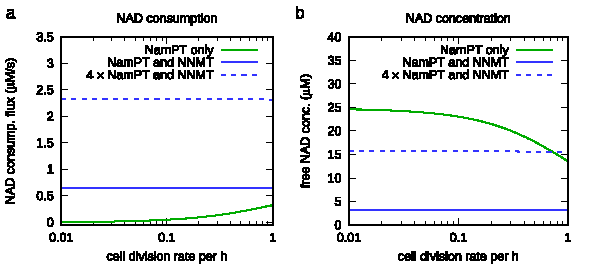
\includegraphics[width=\textwidth]{fig_3_NNMT_NAD_flux}
  \caption{\textbf{NNMT enables high NAD consumption flux.} We used a dynamic model of NAD biosynthesis and consumption (for details, see experimental procedures) to simulate NAD consumption flux. The amount of NMNAT and NamPRT used in the simulations where adjusted such that the free NAD concentrations were in the range reported in the literature. All other enzyme concentrations were set equal. Details are given in supplementary table~S2. In the absence of NNMT (blue lines), steady state NAD consumption rates (A) are higher despite reduced NAD concentrations (B). Increasing the amount of NamPRT in the simulation fourfold (blue dotted lines) partially compensates for the decreased NAD steady state concentration caused by Nam degradation through NNMT.}
  \label{fig:NNMT_NAD_flux}
\end{figure}

\newpage


\subsection{Figure 4}

\begin{figure}[ht]
  \centering
  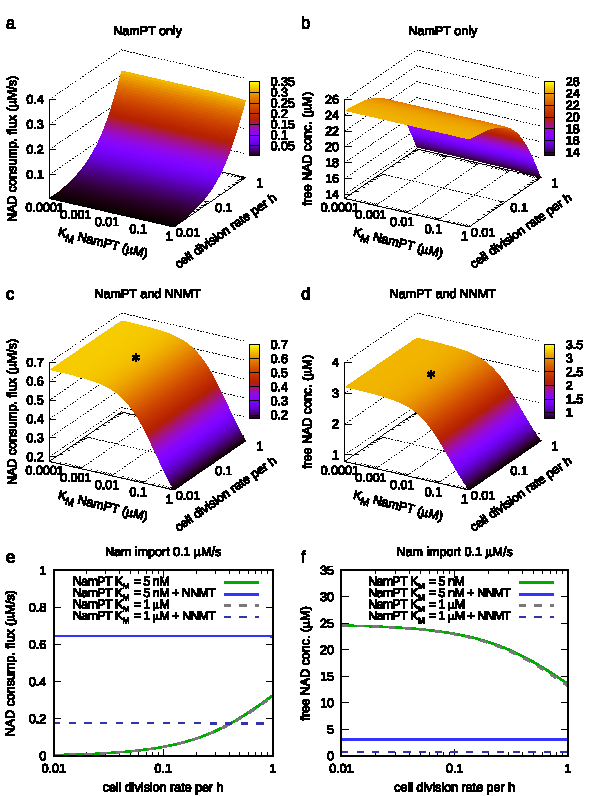
\includegraphics[width=0.9\textwidth]{fig_4_NamPRT_affinity_Nam}
  \caption{\textbf{Role of NamPRT affinity for Nam.} Using the dynamic model of NAD biosynthesis and consumption we simulated the affect of different Michaelis-Menten constants ($K_M$) of NamPRT for Nam on steady state NAD consumption flux and NAD concentration at different cell division rates. All the parameters were equal to those used for the simulations in figure~\ref{fig:NNMT_NAD_flux}. In the absence of NNMT (A and B), the $K_M$ of NamPRT has little influence on NAD consumption and concentration, but both are changing with cell division rates. In the presence of NNMT (C and D), decreasing $K_M$ of NamPRT enables increasing NAD consumption flux and NAD concentration. NNMT furthermore makes both, NAD consumption flux and concentration, almost independent of cell division rates. Comparing the situation with and without NNMT (E and F) at different NamPRT $K_M$ reveals that at low $K_M$ (dashed lines) and high cell division rates NNMT no longer enables higher NAD consumption rates compared to NamPRT alone (green line and dashed black line).}
  \label{fig:NamPRT_affinity_Nam}
\end{figure}

\newpage


\subsection{Figure 5}

\begin{figure}[ht]
  \centering
  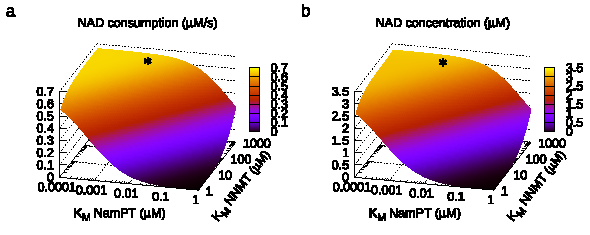
\includegraphics[width=\textwidth]{fig_5_optimal_substr_affinities}
  \caption{\textbf{The substrate affinities of human NNMT and NamPRT are optimal.} Using the same model as in figures~\ref{fig:NNMT_NAD_flux} and~\ref{fig:NamPRT_affinity_Nam}, we simulated the impact of changes in the $K_{M}$ for both NamPRT and NNMT on NAD consumption rates (A) and NAD concentration (B). Both are increasing with decreasing $K_{M}$ of NamPRT but increasing $K_{M}$ of NNMT. The affinities reported for human enzymes (indicated by a black asterisk) appear to be close to optimal, as further improvements would have little or no effect on NAD consumption or concentration.}
  \label{fig:optimal_substr_affinities}
\end{figure}

\newpage


\subsection{Figure 6}

\begin{figure}[ht]
  \centering
  \includegraphics[width=0.75\textwidth]{fig_6_unresolved_loop}
  \caption{\textbf{The function of the structurally unresolved loop structure of NamPRT.} Most Deuterostomia that encode NNMT show a sequence insertion in the N-terminal region of NamPRT that has been revealed by multiple sequence alignment of NamPRT from different species (A). Coloured circles indicate the enzymes present in the respective species blue: NamPRT and NNMT; black: NamPRT, NADA and NNMT; yellow: NamPRT and NADA. For a more comprehensive alignment, please see supplementary figure~S1. The visualisation of human NamPRT (B) is based on a structure prediction of SWISS-MODEL \cite{Arnold2006,Biasini2014} using the model 2H3D of the human NamPRT as template \cite{Wang2006}. The inserted region is not resolved in any of currently available crystal structures of NamPRT and thus appears to be a flexible loop structure at the surface of the NamPRT dimer, coloured in red. Immunofluorescence images show that the localisation of the FLAG-tagged mutant protein lacking the unresolved loop (C) is not changed compared to FLAG-tagged human wildtype NamPRT. Both show a heterogeneous nuclear cytosolic localisation in HeLa S3 cells. \textit{In vitro} measurements using recombinant protein show that the mutant NamPRT has a lower activity than the wildtype enzyme (D) and is not activated by ATP (E). Bars in D) and E) with different letters indicate significant difference of measured values as estimated using a T test assuming independent samples and significance at $p < 0.05$.}
  \label{fig:unresolved_loop}
\end{figure}

\newpage


\subsection{Figure 7}

\begin{figure}[ht]
  \centering
  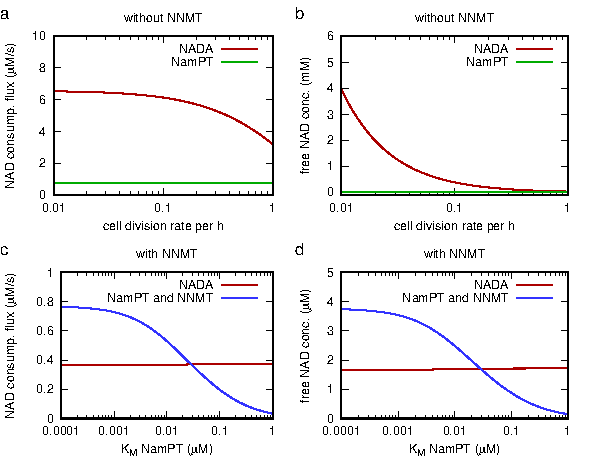
\includegraphics[width=\textwidth]{fig_7_NNMT_comp_advantage}
  \caption{\textbf{NNMT provides a competitive advantage and makes NADA obsolete.} To simulate competition for common resources, we created a two compartment model where one compartment contained NADA but no NamPRT and the other compartment contained NamPRT either with or without NNMT but no NADA. NADA and NamPRT were simulated to be present at equal amounts. In the absence of NNMT (A and B) the compartment containing NADA has slightly lower NAD consumption rates (A) but much higher steady state NAD concentrations (B). In the presence of NNMT, however, both NAD consumption (C) and NAD concentration (D) are lower in the NADA compartment. This effect is dependent on a low NamPRT $K_M$.}
  \label{fig:NNMT_comp_advantage}
\end{figure}

\newpage


\subsection{Figure 8}

\begin{figure}[ht]
  \centering
  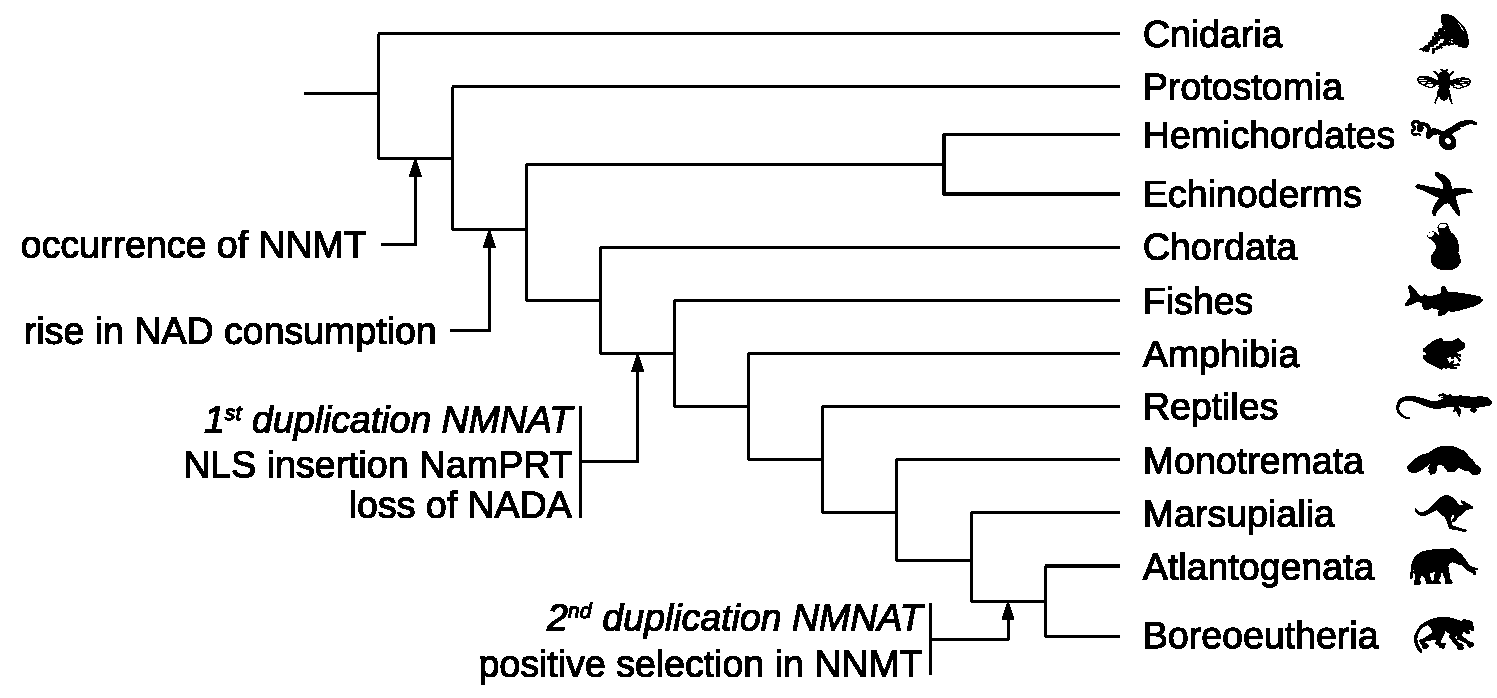
\includegraphics[width=\textwidth]{fig_8_evo_events}
  \caption{\textbf{Schematic representation of evolutionary events in the NAD pathway} Based on the phylogenetic analysis presented here and earlier work \cite{Lau2010} we summarized and indicated important events in the evolution of NAD metabolism in Metazoa. Events in italics are from \cite{Lau2010}. All other events were found in this work.}
  \label{fig:evo_events}
\end{figure}

\todo{What about the positive selection in NNMT?}

\newpage


%%% TeX-master: "manuscript"
% !TeX spellcheck=en_GB

\section*{Supplementary Legends}

\subsection*{Supplementary figure S1}

\textbf{The structurally unresolved loop structure of NamPRT.} Sequence alignment of NamPRT of different species cropped to the region around the unresolved loop structure. Coloured rectangles indicate the enzymes present in the species besides NamPRT; blue: NNMT; black: NADA and NNMT; yellow: NADA; green: NamPRT only. Major clades are indicated for better orientation. Number of amino acid indicated at the top refer to the human protein.


\subsection*{Supplementary figure S2}

\textbf{The phylogenetic distribution of NamPRT and NNMT in birds and reptiles is scattered.}


\subsection*{Supplementary figure S3}

\textbf{Purification of wt NamPRT and $\Delta$42-51 NamPRT.} A) Elution profile of wildtype NamPRT and mutant $\Delta$42-51 on size-exclusion chromatography using a Superdex 200 16/60 column. B) Coomassie stained denaturating SDS-PAGE analysis of $\Delta$42-51 NamPRT (lane 1) and wt NamPRT (lane 2). 3\,$\mu$g of pooled enzyme eluted from SEC loaded onto the gel. C) The column was calibrated with apronitin 6.5\,kDa, ovalbumine 42.7\,kDa, coalbumine 75\,kDa and blue dextran 2000\,kDa. The partition coefficient (Kav) was determined for each standard (light grey squares) and plotted versus log$_{10}$ molecular weight. The Kav was determined for wt NamPRT and $\Delta$42-51 NamPRT and the apparent molecular weight calculated to be 135\,kDa and 110\,kDa, respectively.


\subsection*{Supplementary table S1}

\textbf{Query proteins used for Blast searches.}


\subsection*{Supplementary table S2}

\textbf{Overview of kinetic constants and rate laws used for the construction of the mathematical model.}


\bibliographystyle{plain}
\bibliography{library}

\end{document}
